%%% template.tex
%%%
%%% This LaTeX source document can be used as the basis for your technical
%%% paper or abstract.

%%% The parameter to the ``documentclass'' command is very important.
%%% - use ``review'' for content submitted for review.
%%% - use ``preprint'' for accepted content you are making available.
%%% - use ``tog'' for technical papers accepted to the TOG journal and
%%%   for presentation at the SIGGRAPH or SIGGRAPH Asia conference.
%%% - use ``conference'' for final content accepted to a sponsored event
%%%   (hint: If you don't know, you should use ``conference.'')

\documentclass[tog]{acmsiggraph}
\usepackage[T1]{fontenc}
\usepackage[utf8]{inputenc}
\usepackage[swedish, english]{babel}

%%% Make the ``BibTeX'' word pretty...

\def\BibTeX{{\rm B\kern-.05em{\sc i\kern-.025em b}\kern-.08em
    T\kern-.1667em\lower.7ex\hbox{E}\kern-.125emX}}

%%% Used by the ``review'' variation; the online ID will be printed on 
%%% every page of the content.

\TOGonlineid{45678}

%%% Used by the ``preprint'' variation.

\TOGvolume{0}
\TOGnumber{0}

\title{Perceived Depth Perception In A Virtual Environment Using A Head Mounted Display}

\author{Jesper Blidkvist\thanks{e-mail:Jesper.Blidkvist@live.se}\\Student, BTH}
\pdfauthor{Jesper Blidkvist}

\keywords{Virtual Reality, 3D, Depth Perception}

\begin{document}

%%% This is the ``teaser'' command, which puts an figure, centered, below 
%%% the title and author information, and above the body of the content.

 \teaser{
   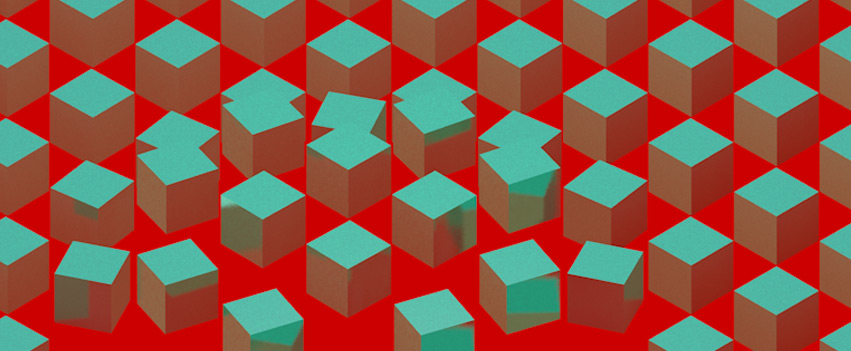
\includegraphics[height=1.5in]{images/temp}
   \caption{BTH 2015, Karlskrona, SE.}
 }

\maketitle

\begin{abstract}
In order to better understand how binocular depth cues can be recreated and manipulated in a virtual environment, a small scale experiment was created in which test subjects where presented with a scene containing a number of cubes. The distance between the two virtual cameras was then either increased or decreased and the test subject was presented with the same scene and asked if they noticed any differences from the previous scene. While the test group was small, there where some indications that a wider distance between the cameras led to the user perceiving the cubes as being further away and smaller, and that a decrease in the distance between the cameras led the test subjects to perceive the cubes as being smaller and closer.



\end{abstract}

\begin{CRcatlist}
  \CRcat{I.3.3}{Computer Graphics}{Three-Dimensional Graphics and Realism}{Virtual Reality}
  \CRcat{H.5.1}{Information Interfaces and Presentation}{Artificial, augmented, and virtual realities};
\end{CRcatlist}

\keywordlist


\copyrightspace

\section{INTRODUCTION}

The purpose of this paper is to investigate how humans perceive depth in a virtual 3D enviroment, more specifically how the distance between the two virtual cameras can influence the users perception of depth. On a pragmatic level, this could be applied in games or other virtual reality mediums to help alleviate the scale issues experienced by some users. The ability to manipulate the users perception without changing the actual geometry of a scene could also be used for example in a multiplayer horror game, where manipulation of the distance between the cameras will cause differences in the perception of the scene, whithout having to change the actual geometry and the experience of the other players.    

There have been a lot of research conducted in regards to human depth perception. There are also a lot of practical examples on how to manipulate our depth perception that can be found for example in art. However, with virtual reality HMDs we are offered an unique opportunity to manipulate a persons depth perception by moving the position of the virtual eyes in such a way that the depth changes. This might have been possible before, using a complicated setup of a number of mirrors but with the HMD the set up of the experiment becomes trivial.  


\section{BACKGROUND}
In order for an observer to perceive an object and ascertain its position relative to the observers own, the brain needs to process and interpret multiple sources of information which are commonly referred to as cues. ~\cite {Reichelt et al:2010:DPHV}. These are often divided into two subcategories, binocular and monocular cues. In some scientific literature the term visual depth cues or pictorial depth cues is used in lieu of monocular cues, for the purposes of this short paper however the terms used will be binocular and monocular cues. As the names suggest, the binocular cues require the use of both eyes while the monocular cues one require one eye.

The binocular cues are a result of the brain taking advantage of the fact that each eye is placed approximately 15 cm apart horizontally on an average human adults head. Because of this the retina of each eye receives a slightly different images as result of the two different viewing angles. These two images are then merged in the striate cortex of the brain, and the difference is interpreted and used as a cue for depth ~\cite{Reichelt et al:2010:DPHV}   From this follows that an object placed at different distances from the observer will have different amounts of binocular disparity due to the images from each eye being different~\cite {Boyd:2000:DPC}. From this it also becomes apparent that as the distance to a given object from the observer increases, the binocular cues will become more and more useless as the images revived by each eye become more and more similar. It is said that binocular cues to work best when the distance to an object is fairly small, approximately 30 meters or less. ~\cite {Palvqvist:2013:DPDS}.

To perceive depth at distances greater than around thirty meters the monocular cues take precedent for most people ~\cite {Palvqvist:2013:DPDS}. The monocular consists of perceived differences in shadows and light on an object 


(2) an object occluding or in other ways hiding one another (3) relative size of similar objects on different distances and so on. (5) the eyes lens level of accommodation, (6) loss of detail with increased distance (8) motion perspective or motion parallax.
%%%/(Kemeny &
Panerai).

It should be noted that one cue does not exclude another and as such a person observing an object at a distance within 30 meters will most likely use a combination of depth cues. ~\cite {Boyd:2000:DPC} . While the cues themselves can be said to be fairly well understood, the way in which they cooperate is somewhat disputed ~\cite {Boyd:2000:DPC} 



\section{EXPERIMENT SETUP}

The experiment was created using the Unity Game Engine developed by Unity Technologies and Oculus Rift HMD and a minimal amount of C\# code to allow the experimenter to change the distance between the virtual cameras with one in game unit at their digression. Unity was chosen as it would allow for a quick experiment set up without the creation of en entirely new engine and since the latest version has native support for the Oculus HMD the interaction between the software running the experiment and the HMD will not pose a problem.

At the time of writing there are a number of HMDs avaliable for developer, the Oculus was chosen primarily for its native support in Unity and that it was easily avaliable for the experimenter.

The scene created in unity consists of a blue skybox, a plane and seventy five cubes that are generated and randomly placed within a random distance from 0.0.0, although no less then -10 in game units or  more then 10 in game units at start-up. The experimenter then controls the distance between the cameras using the arrow keys, the left one decreases the distance with one in game unit, and the right one increases it with one in game unit. To alleviate possible sources of nausea, a script was written that disables the rendering och the cubes if desired so that the experimenter can change the distance between the cameras greatly without the experimentee noticing. 

During the actual experiment the user is seated on a chair and the HMD is placed on their head. The user is then presented with the previously mentioned scene. The test subject will then be asked to look at the cubes for about thirty seconds before the the experimenter will disable the rendering of the cubes. When this avtion has been performed, the distance between the cameras will then be increased, and the test subject will again be presented with the scene and asked to observe for 30 seconds and asked if they notice any difference from the previous scene.  

\section{RESULT}

The title, author, and affiliation information should be centred
above the body of your content. The title should be set in a 14-point
bold sans-serif typeface with 18-point line spacing. The author and
affiliation information should be set in a 10-point serif typeface
with 12-point line spacing.

The title should be appropriately capitalized. ``All caps'' is not
appropriate. The following link provides assistance with appropriate
capitalization:

{\small\url{http://www.grammarbook.com/punctuation/capital.asp}}

Affiliations should include your educational institution or employer's
name, and a valid e-mail address.

\section{FUTURE WORK}

This experiment focused on only one depth cue. 




\section{Contact Information}

If you have questions or suggestions regarding this document, please
contact Jesper Blidkvist at ``Jesper.Blidkvist@live.se''.

\section*{Acknowledgements}

Tack till inte en jävel

\bibliographystyle{acmsiggraph}
\nocite{*}
\bibliography{template}
\end{document}
